\documentclass[preprint,10pt,authoryear]{elsarticle}
\linespread{1.25}

\usepackage[dvipsnames]{xcolor}
\usepackage[round]{natbib}
\usepackage{graphicx}
\usepackage{amsmath}
\usepackage{lscape}
\usepackage{placeins}
\usepackage{breqn}
\usepackage{threeparttable}
\usepackage{longtable, threeparttablex}
\usepackage{amsfonts}
\usepackage{eurosym}
\usepackage{colortbl}
\usepackage{numprint}
\usepackage{lipsum}
\usepackage[tableposition=top]{caption}
\usepackage{booktabs}
\usepackage{float}
\floatstyle{plaintop}
\restylefloat{table}
\usepackage[T1]{fontenc}
\usepackage{afterpage}
\usepackage{tabularx}
\usepackage{array}
\usepackage{multirow}
\usepackage{pdflscape}
\usepackage{subcaption}
\usepackage{geometry}
\usepackage{setspace}
\usepackage{stackengine}
\usepackage{lineno}
\usepackage{rotating}
\usepackage{changes}
\usepackage{hvfloat}
\setcounter{secnumdepth}{4}
\setcounter{tocdepth}{4}
\usepackage[colorlinks,citecolor=blue,urlcolor=blue,bookmarks=false,hypertexnames=true]{hyperref} 
\usepackage{tikz}
\usepackage{comment}
\usepackage{pdfpages}
\usepackage[utf8]{inputenc}
\usepackage[english]{babel}
\usetikzlibrary{calc}
\usepackage{array}


\tikzstyle{block} = [rectangle, draw, text centered, rounded corners, minimum height=3em]
\tikzstyle{line} = [draw, ->, shorten >=1pt]

\journal{Expert Systems with Applications}

\newcommand{\revision}[1]{\textcolor{red}{#1}}

\AtBeginDocument{
    \renewcommand{\sectionautorefname}{Section} 
    \renewcommand{\subsectionautorefname}{Subsection} 
    \renewcommand{\subsubsectionautorefname}{Subsection} 
}

\geometry{footskip=120pt}

\captionsetup[table]{position=below}

\begin{document}

\section{Introduction}

\revision{Personal} Peer-to-Peer (P2P) lending, in its facet as profit-driven crowdfunding, has progressively emerged as a compelling alternative to the traditional banking system. While P2P lending platforms mirror certain characteristics of traditional banks, they deviate substantially in terms of the financial products offered and their operational mechanisms. For instance, these platforms are mainly characterised through an online business model and chiefly provide medium-term financial solutions, generally accommodating maturities of up to 5 years \citep{coakley2020p2p}.

A distinguishing aspect of P2P lending lies in its ability to democratize access to credit. The traditional banking system, characterized by stringent credit approval processes, often poses barriers for potential borrowers to quickly access funding. In contrast, P2P lending platforms commonly simplify the borrowing process, thereby improving credit access. This disparity can be seen  as instrumental for the growing adoption of P2P lending platforms.

The platforms commonly promote the offer of a win-win scenario for both lenders and borrowers. Borrowers gain access to easy-accessible credit, while lenders obtain an opportunity to earn higher returns, establishing a platform for mutual profitability \citep{malekipirbazari2015risk}. This distinctive attribute, coupled with a rapidly scaling online business character for most P2P lending platforms, has spurred a substantial surge in the issuance of P2P loans in recent years.

However, limited access to traditional credit data for P2P lending platforms, compared to banks, further amplifies the degree of information asymmetry between lenders and borrowers \citep{duarte2012trust}, potentially escalating the default risk for loans on these platforms. \revision{Our study is motivated by an essential difference in the risk ownership of traditional bank lending compared to P2P lending. This difference manifests in the constellation that in traditional lending, banks provide credit scores for borrowers and also bear the risk of the loan defaulting in case of a borrower not being able to redeem the debt. Hence, the incentive to provide accurate credit scoring lies in the interest of the bank as it also incurs the risk of default. Conversely, in P2P lending the scoring of credit risk is conducted by the P2P lending platform but the default risk of the loan is fully born by the lender that issues the credit \citep{giudici2019network,havrylchyk2018financial}. This misalignment can lead to the flaw of inaccurate credit score provision as P2P lending platforms are primarily incentivised to expand credit volume whereas lenders hold primary interest in accurate credit scores. In this realm it becomes clear that P2P lending lacks the traditional mechanisms of credit risk control present in conventional banking systems. Thus, we strive to enrich the ongoing academic discourse around modelling credit scores in P2P lending markets \citep{lyocsa2022default,chen2021predicting,niu2020resampling,giudici2019network,giudici2020network,chen2022network,liu2022two,lee2021graph}.} The majority of the literature on modelling credit default risk in P2P lending markets has focused on traditional credit risk \revision{factors} without taking into account the intricate network structures of these platforms \revision{through network centrality metrics}. In this context, it appears crucial to point scholarly attention to the usage of alternative data sources and innovative credit risk modelling approaches that could improve the accurate prediction of loan defaults in P2P lending markets. Therefore, in this study we propose an enhanced two-step \revision{machine learning (}ML) modeling process that utilises network analysis in the first step and consecutively combines derived network-based centrality metrics with conventional credit risk factors to improve loan default classification.

\revision{Our study leverages data from Bondora, a European P2P lending platform, which has been active since 2009 in Estonia, Finland, Spain, and Slovakia. The platform boasts funds from $225,837$ individual lenders and has disbursed \euro{867.5 Mio}. in loans\footnote{\url{https://www.bondora.com/en}}}. We focus on six network centrality measures PageRank \citep{brin1998anatomy}, betweenness centrality \citep{freeman1977set,freeman2002centrality}, authority score \citep{kleinberg1999hubs}, katz centrality \citep{katz1953new}, hub centrality \citep{kleinberg1999hubs}, and closeness centrality \citep{sabidussi1966centrality}, which we hypothesize to have a substantial impact on loan default prediction. To evaluate the performance of our approach, we utilize three ML models: Elastic Net (EL) \citep{zou2005regularization}, Random Forest (RF) \citep{breiman2001random}, and Multi-Layer Perceptron (MLP) \citep{goodfellow2016deep} with varying hyper-parameter and factor configurations to rigorously assess the influence of the network centrality measures on the model prediction accuracy. Subsequently, a feature importance analysis is conducted to determine the individual contribution of the six centrality features within the model performance and compare their relative importance across the three models.

By proposing this enhanced two-step approach to loan default prediction in personal P2P lending, our study aims to make a significant contribution to the field of credit risk modelling. \revision{Through the integration of graph theory into our modeling approach, we aim to capture a loan's position and similarity in contrast to other loans within the broader network. Such information can impact the credit risk assessment for several reasons: I.) the similarities of various loans captured by the network centrality measures can capture latent features which we do not observe directly, thus adding additional information to the loan default classification. II.) the similarity degree, how similar a loan contract is with others, can affect the platform's ability to accurately score the respective loan. If we consider the context of a new borrower applying for a loan and the loan's profile is very dissimilar to any of the other loan contracts that the platform has seen, it may raise difficulties for the platform to accurately score the particular loan contract. III.) Hence, the inclusion of network centrality measures may also provide a reflection of a loan's similarity to the entire loan pool of the P2P platform, where higher levels of loan similarity with solvent loans can imply a higher level of collateralized risk. A borrower with a high degree of similarity to previous non-defaulted loans may have a stronger likelihood to repay the loan, thereby potentially lowering the default risk for the lender. This nuanced information would not become available in traditional credit risk assessment tools. Thus, our incorporated network-related measures could provide an additional layer of understanding to enhance the loan default prediction process. Through our comparative study design we further aim to uniformly assess the effect of incorporating network centrality measures into credit scoring models of varying complexity. By choosing three different ML models, belonging to the class of statistical, tree-based, and deep learning methods, we aim to provide holistic evidence on the suitability of graph-based credit risk modeling in P2P lending markets. Our findings indicate that the inclusion of network-based centrality measures, across all model types, significantly improves the loan default classification of the scoring models. The results remain robust under the utilisation of randomly shuffled dummy centrality measures and confirm our initial findings.} Insights derived from this study should guide practitioners to improve their credit risk assessment processes and decision-making in P2P lending to grant more stable lending conditions. 

The remainder of this paper is organized as follows. \autoref{Literature Review}, outlines the existing literature on credit default prediction, the methodical process transition to ML \revision{and the role of graph-based network models in risk estimation.} We also identify research gaps in the current literature and introduce the foundations of our methodological approach. The methodological framework, presented in \autoref{Methodology}, introduces our proposed two-step ML methodology, embeds it in the concept of graph theory, and outlines the process of network construction. It further describes the statistical- and ML models applied in our study and outlines the metrics used for the model evaluation. In \autoref{Data}, we describe the dataset used for our analysis, detailing its source, variables, and pre-processing steps. \autoref{Results} presents the empirical findings of our study, including the feature importance analysis and model performance comparison. It further constitutes of the robustness checks and provides implications for P2P lending platforms and borrowers alongside the limitations and potential biases of our study approach. Finally, our conclusion in \autoref{Conclusion} summarizes the main findings of this study and points to potential future research directions.

\section{Literature Review}
\label{Literature Review}
\subsection{\revision{Credit Risk and Default Prediction}}
\revision{One of the major frontiers in modern finance is the quantification of credit risk \citep{kealhofer2003quantifying}. Since the inception of the famous Black-Scholes model \citep{black1973pricing} for pricing equity derivatives, new approaches of modeling inherent default risk in conventional credit have continuously evolved. Following the foundational works of \cite{altman1968financial} and \cite{merton1974pricing}, various statistical methods such as Multiple Discriminant Analysis (MDA) \citep{altman1968financial}, binary quantile regression (BQR) \citep{li2010hybrid}, probit analysis \citep{dierkes2013business} and logistic regression \citep{crook2007recent,abdou2008neural,verbraken2014development} have been proposed to predict credit default risk. However, with advancements in computer technology these modeling concepts got rivaled by more complex analytical techniques originating from the field of ML, capable to handle large data sets with multiple dimensions. Non-parametric models like Artificial Neural Networks (ANN) \citep{babaei2020multi}, Gradient Boosting Machines (GBM) or extreme gradient boosting (XGBoost) \citep{tian2020credit,li2018heterogeneous}, adaptive boosting algorithms (AdaBoost) \citep{onan2016multiobjective}, support vector machines (SVM) \citep{bellotti2009support,barboza2017machine}, and random forest models \citep{malekipirbazari2015risk} are found to have yielded superior classification accuracy in estimating credit default over conventional statistical techniques. Similarly, studies have also applied deep learning models like multi-layer perceptrons (MLP) \citep{angelini2008neural,battiston2012debtrank}, long-short-term memory (LSTM) \citep{shen2021new}, and probabilistic neural networks (PNN) \citep{huang2018enterprise}, which have shown considerable accuracy over traditional statistical models in default prediction. Congruently, within the context of our study we place further focus on scholarly work that has specifically explored the application of ML in credit default prediction.}

\subsection{\revision{Credit} Default Prediction using ML}
In the realm of traditional banking and corporate lending, several studies have successfully employed ML models for default prediction \citep{barboza2017machine,garcia2019exploring,ghatasheh2014business,huang2004credit, bellotti2009support,lessmann2015benchmarking}. \cite{huang2004credit} made an early contribution by comparing the performance of different non-paratmetric ML models, including ANNs, decision trees, and SVMs, in predicting bond defaults, thereby showcasing that the relative importance of financial input variables differed substantially across the different ML methods. Similarly, \cite{lessmann2015benchmarking} conducted an extensive comparison of 41 different classifiers, providing a comprehensive benchmark for credit scoring and modelling approaches. The authors showcased in their comparative analysis that several classifier, specifically heterogeneous ensemble classifiers, predict credit risk significantly more accurate than the industry standard logistic regression model. \cite{bellotti2009support} investigated SVMs on a large credit dataset and found SVMs to be effective in classifying defaulting credit card customers, requiring a notable number of support vectors for optimal performance. Studies by \cite{barboza2017machine} and \cite{garcia2019exploring} specifically focus on the study of credit risk as a binary classification problem and apply ML classifier models to assess the default prediction accuracy in restrictive conditions such as high variable correlation, outliers, and missing values \citep{barboza2017machine} or a varying distribution of sample types from data \citep{garcia2019exploring}. Both studies find that ML models can provide improvements in predictive utility of scoring models.

Within the literature \revision{a considerable strand further stressed the importance of network models in assessing credit risk particularly in the context of complex and interlinked modern financial systems \citep{allen2009network,angelini2008neural,battiston2012debtrank}.} The interconnected nature of these systems implies that an individual entity's failure can precipitate cascading effects on others, underscoring the utility of network models for capturing such dynamics.
In the context of credit default prediction for private, corporate and financial entities, scholars applied neural network techniques to estimate credit default in various settings. In a seminal work, \citet{galindo2000credit} applied neural networks to predict the likelihood of default in consumer loans. By analyzing a set of socio-economic variables along with traditional financial metrics, their neural network model was able to identify complex interactions that significantly impact the risk of default. Subsequent studies on consumer loan default prediction focus on optimising the application of neural network techniques for predicting default \citep{Babaev2019rnn, dastile2021making, iwai2020structured}. Other studies as in \cite{angelini2008neural} conceptualized feedforward neural networks for predicting loan default in corporate settings and validly classified corporate loan default \revision{with enhanced accuracy}. Further scholarly work focused on the application of specific deep learning models on corporate loan default prediction such as artificial neural networks \citep{leong2016credit}, LSTM \citep{shen2021new}, or PNN \citep{huang2018enterprise}. More recently, studies by \cite{poenaru2022default} and \cite{kou2021bankruptcy} considered the utilisation of neural network techniques under the specific usage of network-based features to extract additional information from a network structure of financial performance data for small- and medium-sized enterprises (SMEs) to predict firm default.

While these studies have made significant strides, they have primarily been focused on specific alternative- or traditional risk factors in the feature engineering process. Recently, there has been a growing recognition for the need to consider additional factors and techniques, \revision{specifically when aiming to capture complex nonlinear relationships among the credit features and credit risk \citep{huang2014kernel}. Hence, complex network-based modeling techniques may promise advanced feature engineering to fully mine dependency relationships among the variables, which requires further exploration.}

\subsection{Graph-Based Scoring Models \revision{and Their Application in P2P Lending}}

\revision{The field of network analysis  and graph-based modeling has recently shifted its focus} on the application of network analysis in the context of credit default prediction. Scholars have been concerned with clarifying the role of network importance and enriching the pool of informative features to more accurately predict credit default. \revision{Early} studies have documented the important role of relational networks in lending markets. \cite{garmaise2003informal} provide first evidence of the informative role that informal networks play in establishing access to \revision{credit} finance in the U.S. commercial real estate market. \revision{Later} studies have emphasised the positive influence of personal networks in the formation of interest rates for loan issuance \citep{engelberg2012friends}, and decisions on credit allocation in corporate settings from banks to firms \citep{haselmann2018rent}. \cite{stanton2018mortgage} \revision{are among the first to} empirically proof the importance of a firm's network position, showcasing that the loan default rates of a firm and its comparative performance are related to the relative position of the respective company against its industry peers within the considered network. \revision{Further studies on systemic risk transmission and contagion among financial institutions \citep{constantin2018network,torri2018robust} highlight the benefit of structural information in graphs or networks that indicate latent factors irretrievable from conventional modeling approaches.}

\revision{This} evidence points to the influence of network effects within lending networks and consequently raises the case to consider them in the classification of default scenarios for financial \revision{entities \citep{kou2021bankruptcy,yildirim2021big,sukharev2020ews,zhou2023forecasting,shi2024improved}}. \revision{\cite{kou2021bankruptcy} utilise network information derived from payment networks of SMEs, where nodes represent firms and edges indicate common payment transactions, to predict corporate default. The gathered topological information proves transactional data to improve SME bankruptcy prediction. In turn, \cite{yildirim2021big} further advances this network modeling approach by deriving graph centrality metrics and comparatively assessing statistical and tree-based credit scoring models on a data set of Turkish companies. The findings reveal a uniform improvement across all graph-enhanced model ROCs in contrast to their conventional peers. \cite{sukharev2020ews} coincide in this finding and report that graph-induced transactional information significantly improves the prediction accuracy of the neural networks in classifying loan defaults of bank customers. } \revision{Conversely, studies focusing on credit default prediction in consumer lending find similar evidence for the utility of graph-topological information in the credit risk modeling process. \cite{zhou2023forecasting} apply graph-attention-based networks to model consumer credit risk under the influence of complex inter-relationships stemming from the credit providers' users. The approach results in superior prediction accuracy for the graph-based model over standard ML techniques. \cite{shi2024improved} apply a hybrid graph neural network (GNN) approach combined with k-nearest-neighbour (KNN) to perform the graph transformation in an unsupervised way to enhance loan default prediction. Their superior classification accuracy over conventional ML models emphasis the benefit of constructing links between observed instances prior to the modeling process to further exploit latent information in the credit data.}

In the context of peer-to-peer (P2P) lending platforms, the application of advanced ML models under the utilisation of network features has been a young but increasingly recognized research field. Several studies \revision{ have focused} on the prediction of loan default in P2P lending \citep{lyocsa2022default, chen2021predicting,giudici2019network,giudici2020network,chen2022network,ahelegbey2019factorial,ahelegbey2019latent,liu2022two,lee2021graph} but only some \citep{giudici2019network,giudici2020network,chen2022network,ahelegbey2019factorial,ahelegbey2019latent} have leveraged network effects \revision{measured by centrality measures} to predict loan defaults. \revision{\cite{giudici2019network,giudici2020network} employ graph-based centrality features, namely PageRank and degree centrality in their effort to predict loan defaults in SME-focused P2P lending through similarity networks. The inclusion of the topological variables is found to increase the predictive performance of the methods employed. \cite{ahelegbey2019factorial,ahelegbey2019latent} coincide in this matter and apply network-based modeling techniques on an SME loan sample to retrieve latent community information. By utilising topological features, namely degree centrality in a single value decomposition (SVD) framework, the authors create a factor network-based approach to segment companies into homogeneous clusters using logistic-type models, thereby approving their enhanced default prediction accuracy. Conversely, \cite{chen2022network} are first to investigate the effect of including degree, betweenness, and eigenvector centrality in the credit default modeling process for personal P2P lending, using logit regression. The authors find that the position of a lender within the network, classified by the topological features does positively contribute to the classification of default risk.} \revision{From this review, we determine the following gap in the literature on credit default prediction in personal P2P lending: i) no scholarly effort so far has systematically investigated the effect of including network topological features in credit scoring models within a comparative setting to arrive at a uniform conclusion. ii) The varying complexity of different scoring models has not been accounted for in previous studies, which leaves uncertainty about the concrete effectiveness of including network topological features in the credit default classification process. Hence, we strive out to investigate this conundrum in the following sections of this study.}

\section{Methodological Framework}
\label{Methodology}

We describe a two-step modeling approach designed to capture and analyze the complex interactions of loans to predict default probability based on initial credit features and \revision{centrality measures} under the use of different ML models. Our first step \revision{consists of constructing} a network based on loans. The development of this network involves systematically representing the loans as nodes and their interactions as edges. From this network, we then extract graph features that effectively summarize the structural characteristics of the loans and their interactions. The second step involves using these graph features and initial features as inputs to train the three ML models. Finally, to ensure that our results are robust and reliable, we make use of several model evaluation metrics. We begin with commonly used ML metrics such as accuracy, precision, recall, and the F1 score. To compare the performance of models based on dataset with and without graph features, we also use the DeLong Test.

\subsection{Step 1: Network Construction and Centrality Feature Extraction}
\label{subsec: Network Construction}

\subsubsection{Process of Network Construction on Loans}
\label{subsubsec: Process of Network Construction on Loans}
\revision{Our} network construction methodology draws on previous work in social network analysis, particularly in the context of financial systems \citep{newman2003structure, glasserman2015net, Battiston2016}.

We opt for an undirected weighted network, as the relationship between two \revision{loans} sharing common attributes does not involve a directionality, while we still need weights to express the distance or similarity among \revision{loan contracts}. We use vector $X_i = (x_{i1}, x_{i2}, \cdots, x_{ip},\cdots, x_{iP})'$ to denote node $i$, where $x_{ip}$ is the $p$-th feature among the total $P$ features of this loan.

\revision{First,} a fully connected graph \revision{is built} and \revision{subsequently} reduced to its minimum spanning tree (MST). For the fully connected graph, there is an edge between any pair of nodes. We assign weights to every edge by calculating the Gower's distance \citep{gower1971general} between two nodes. Gower's distance is a metric that effectively measures dissimilarity between observations for mixed data types, including continuous and categorical features. It normalizes the differences within each feature to a 0-1 scale, allowing meaningful comparison across disparate data ranges. This metric accommodates variables with different scales and is not influenced by the range of features. For each pair of \revision{loans} $i$ and $j$, we calculate the Gower's distance $d_{ij}$ as follows:
\begin{align*}
d_{ij} = w_{ij} &=\sum_{p=1}^{P} \frac{1}{P} \times \frac{d^p_{ij}}{\text{max}(x_{\cdot p}) - \text{min}(x_{\cdot p})}, \\
\text{where } d^p_{ij} &= \left\{
  \begin{array}{ll}
    |x_{ip} - x_{jp}| & \text{if } x_p \text{ is a continuous variable}, \\
    1 & \text{if } x_p \text{ is a categorical variable and } x_{ip} \neq x_{jp}, \\
    0 & \text{if } x_p \text{ is a categorical variable and } x_{ip} = x_{jp}.
  \end{array}
\right.
\end{align*}

We then reduce this fully connected graph to its MST \citep{kruskal_shortest_1956,prim_shortest_1957} and extract the graph. In the fully connected graph, all graph features will be the same across all loan contracts, while with the MST, we take the most connected sub-graph and extract information efficiently \citep{giudici_2020_network}.

\subsubsection{Network Centrality Features Used in the Analysis}
\label{subsubsec: Graph Features Used in the Analysis}
Our analysis of \revision{loan} interconnectedness within the constructed network was based on several centrality measures, each contributing to a comprehensive understanding of borrower behavior and influence in the network. Here we assume there are $N$ nodes in the graph and detail each centrality measure:

\paragraph{Degree Centrality ($C_D(X_i)$)}
This metric quantifies the number of direct connections a node has in the network. It encapsulates the immediate risk exposure or influence of a given node. A node with high degree centrality is typically heavily involved in the network's interactions, implying a more significant role or potential vulnerability. Mathematically, it is expressed as $C_D(X_i) = \sum_{j=1, j \ne i}^N a_{ij}$, where $a_{ij}$ denotes the adjacency between node $X_i$ and $X_j$ \citep{freeman_2002_centrality}.

\paragraph{Closeness Centrality ($C(X_i)$)}
This metric calculates the average length of the shortest paths to reach all other nodes in the network from a given node. It captures how quickly information can propagate from a given node to others. Formally, it is represented as $C(X_i)=\frac{1}{\sum_{j=1, j \ne i}^N d(X_i, X_j)}$, where $d(X_i, X_j)$ represents the shortest-path distance from $X_i$ to $X_j$ \citep{freeman_2002_centrality}.

\paragraph{Betweenness Centrality ($C_B(X_i)$)}
This measure captures the influence of a node over the flow of information between other nodes in the network. \par It is computed as $C_B(X_i)=\sum_{j,k \in \{1,2,\cdots, N\}}\frac{\sigma(X_j,X_k|X_i)}{\sigma(X_j, X_k)}$, where $\sigma(X_j, X_k)$ is the total number of shortest paths from node $X_j$ to node $X_k$, and $\sigma(X_j,X_k|X_i))$ is the number of those paths passing through node $X_i$ \citep{freeman1977set}.

\paragraph{PageRank ($PR(X_i)$)}
\revision{Our} PageRank \revision{variable} evaluates the importance of nodes based on the quality of incoming links. It is defined as $PR(X_i)=(1-d)+d\sum_{X_j \in M(X_i)}\frac{PR(X_j)}{L(X_j)}$, where $M(X_i)$ is the set of pages that link to $X_i$, $L(X_j)$ is the number of outbound links on page $X_j$, and $d$ is a damping factor, usually set to $0.85$ \citep{brin1998anatomy}.

\paragraph{Katz Centrality ($C_{\text{Katz}}(X_i)$)}
Katz Centrality considers both direct and indirect influence of a node's neighbors. It is represented as $C_{\text{Katz}}(X_i)=\sum_{j=1}^{N}\beta A_{ij}C_{\text{Katz}}(X_j)+\alpha$, where $A_{ij}$ denotes the adjacency matrix element, $\beta$ is a scaling factor, and $\alpha$ is a constant term representing the node's intrinsic centrality \citep{katz1953new}.

\paragraph{HITS Algorithm (Authority Score $a(X_i)$ and Hub Score $h(X_i)$)}
The HITS (Hyperlink-Induced Topic Search) calculates the authority and hub scores for a node based on its incoming and outgoing links, respectively. The Authority Score $a(X_i)$ is computed as the sum of the hub scores of each node $X_j$ that points to $X_i$, i.e., $a(X_i)=\sum_{X_j \in M(X_i)}h(X_j)$, where $M(X_i)$ is the set of nodes that point to $X_i$ and $h(X_j)$ is the hub score of node $X_j$. Similarly, the Hub Score $h(X_i)$ of a node $X_i$ is computed as the sum of the authority scores of each node $X_j$ that $X_i$ points to, i.e., $h(X_i)=\sum_{X_j \in N(X_i)}a(X_j)$, where $N(X_i)$ is the set of nodes that $X_i$ points to and $a(X_j)$ is the authority score of node $X_j$ \citep{kleinberg1999hubs}.


\subsection{Step 2: ML Models}
\label{subsec: ML Models}
For the second step of our \revision{methodology}, we introduce several ML techniques. \revision{We employ EN, RF, and MLP models} due to their reliant estimation and processing power as well as convenient interpretability. \revision{A grid search algorithm is further employed} to fine-tune \revision{the} hyperparameters \revision{of each model}. In the following subsection, we will briefly introduce each model \revision{specification} and focus on its hyperparameter settings. For the process of the model application, we use the H2O platform \citep{h2o2017} as fully integrated estimation tool to train the models.

\subsubsection{Elastic Net (EN)}
\label{subsubsec: Elastic Net (EN)}
We \revision{apply} the EN\footnote{For detailed elaborations on the technical notation of the EN please refer to \ref{GLM_model_specificity}.}, facilitated by \revision{a} Generalized Linear Estimator (GLM), as initial ML model. The EN, originally proposed by \citet{zou2005regularization}, is an advantageous regularization and variable selection method, integrating the strengths of both L1 and L2 penalties, synonymous with Lasso and Ridge regression respectively. \revision{We opt to implement the EN model over the standard logistic regression because the modelling technique is found to perform better in two-class classifications tasks with any consistent loss functions \citep{zou2005regularization}. Furthermore, the EN conducts automatic feature selection with the ability to perform grouping, in contrast to penalized logistic regression that applies either univariate ranking or recursive feature elimination \citep{zhu2004classification} to reduce the number of features in the final model.} \revision{Hence, the EN} provides an effective balance between bias and variance, addressing potential overfitting issues and ensuring model generalizability. Particularly for our dataset, it \revision{also} aids in the recognition of key predictive features linked to loan default.

The $\alpha$ parameter governs the mixing proportion of the L1 and L2 penalties, with values ranging from 0 (only Ridge penalty) to 1 (only Lasso penalty). As such, an $\alpha$ hyperparameter space of $\{0, 0.2, 0.4, 0.6, 0.8, 1\}$ is defined. Concurrently, the $\lambda$ controls the overall strength of the penalty, with a larger $\lambda$ leading to more regularization and feature selection. We specify a diverse range of lambda values to cover different degrees of regularization, setting $\lambda \in \{1e-4, 1e-3, 1e-2, 1e-1, 1, 10, 100\}$. This comprehensive grid search of hyperparameters aids in identifying the optimal model specification with regards to our credit risk data.

The model estimation is executed under a binomial family setting to suit the binary nature of our loan default outcome.

\subsubsection{Random Forest (RF)}
\label{subsubsec: Random Forest (RF)}
RFs, introduced by \cite{breiman2001random}, have emerged as a robust and versatile ML method with excellent performance across a diverse range of applications. The non-parametric nature of these models makes them exceptionally capable of handling high-dimensional spaces and intricate interactions. In the realm of credit risk modeling, the RF algorithm is particularly effective, given its ability to model complex non-linear relationships between predictors and the probability of loan default, thereby making it a potent tool for default prediction \citep{lessmann2015benchmarking}.

In this study, we employ a random forest model\footnote{For detailed elaborations on the technical notation of the RF please refer to \ref{RF_model_specificity}.} using a distributed and paralleled implementation of the \revision{RF} algorithm for maximum efficiency. The model is configured with varying hyperparameters - \texttt{ntrees} and \texttt{max.depth}. \texttt{ntrees} defines the number of trees in the forest, with range $\{50, 100, 150, 200, 250\}$. \texttt{max.depth} stipulates the maximum depth of each tree in the forest, with range $\{5, 10, 15, 20\}$.

\subsubsection{Multi-Layer Perceptron (MLP)}
\label{subsubsec: Multi-Layer Perceptron (MLP)}
\revision{To further account for} the complexity and the latent interconnectedness of credit data, we employ a deep learning approach in the form of a MLP. Deep learning methods enable models to automatically learn representations of data through the use of neural networks with multiple layers \citep{lecun2015deep}. MLP, a specific type of deep feed-forward ANN, consists of multiple layers of nodes: an input layer, one or multiple hidden layers, and an output layer. In line with the predictive power of deep learning models reported in the literature \citep{sadhwani2021deep}, we anticipate that the MLP model, through its ability to model intricate structures in high-dimensional data, could offer meaningful insights and improved prediction accuracy in the context of credit risk modeling.

For our MLP model\footnote{For detailed elaborations on the technical notation of the MLP model please refer to \ref{DL_model_specificity}.}, the input layer is adjusted according to the number of features ($P$) of each observation to reach at a different number of neurons. The output can only have one neuron with softmax \citep{rumelhart1985learning} as activation function, outputting a value between 0 and 1 as the probability of default. We focus on \texttt{hidden} layers with range $\{[50, 50], [100, 100], [200, 200],\}$ $\{[100, 200, 100], [200, 100, 200]\}$. The \revision{count of individual} numbers in each square bracket represent the number of hidden layers, and the value of each number represents the \revision{amount of} neurons in this layer. For instance, $[100, 200, 100]$ indicates that this MLP contains an input layer, three hidden layer and an output layer. There are $100, 200, 100$ neurons for the 1st, 2nd and 3rd hidden layer, respectively. The hyperparameter \texttt{epochs} controls the time of the weights to be updated to minimize the loss function, with range $\{10, 50, 100\}$.

\subsection{Model Evaluation}
\label{subsec: Model Evaluation}

\subsubsection{General Machine Learning Performance Metrics}
\label{subsubsec: General Machine Learning Performance Metrics}
In this section we outline the main evaluation metrics used in this study to measure the performance of the EN, RF and MLP. In a binary classification task, we have the following confusion matrix \citep{gupta2022deep}: 

\begin{table}[H]
\centering
\begin{tabular}{l|c|c|}
\cline{2-3}
& \multicolumn{2}{c|}{Predicted} \\ \hline
\multicolumn{1}{|l|}{Actual} & Positive & Negative \\ \hline
\multicolumn{1}{|l|}{Positive} & True Positive (TP) & False Negative (FN) \\ \hline
\multicolumn{1}{|l|}{Negative} & False Positive (FP) & True Negative (TN) \\ \hline
\end{tabular}
\caption{Confusion matrix.}
\label{fig:confusion_matrix}
\end{table}





Several additional metrics at the forefront accuracy, precision, recall, and F1-score that are commonly used measures to provide a more comprehensive view of the model's performance \revision{are employed}. Each method is explained below:

We utilise accuracy to assess the performance of a classification model. It measures the proportion of total correct predictions (both positive and negative) out of all predictions made. Mathematically, accuracy is calculated as the sum of True Positives (TP) and True Negatives (TN) divided by the sum of True Positives (TP), True Negatives (TN), False Positives (FP), and False Negatives (FN). $\text{Accuracy} = \frac{\text{TP + TN}}{\text{TP + TN + FP + FN}}$.

Precision (also known as positive predictive value) measures the proportion of true positive predictions among all positive predictions. It is calculated as: $\text{Precision} = \frac{\text{TP}}{\text{TP + FP}}$.

Recall \revision{or sensitivity} measures the proportion of true positive predictions among all actual positives and is calculated as: $\text{Recall} = \frac{\text{TP}}{\text{TP + FN}}$.

The F1-score is the harmonic mean of precision and recall, acting as a balance of these two metrics. It is particularly useful when dealing with imbalanced data and conversely computed as: $\text{F1-score} = 2 \cdot \frac{\text{Precision} \cdot \text{Recall}}{\text{Precision} + \text{Recall}}$

These metrics can help assess the model's performance more accurately, particularly in cases where the original class distribution is uneven \citep{powers2020evaluation}. Each of these metrics offers a distinct perspective on the model's performance and allows us to  draw a collective assessment of the models' predictive capabilities in this study.

In addition, we use the Area Under the Receiver Operating Characteristic curve (AUC-ROC) \citep{fawcett2006introduction} as additional measure to visually compare the model performances. The ROC curve plots the true positive rate against the false positive rate at various threshold settings, while the AUC quantifies the overall performance of the classifier. An exemplary AUC of 0.5 suggests no discrimination, i.e., the model has no ability to distinguish between the positive and negative classes. Conversely, an AUC of 1.0 signifies perfect discrimination.

\subsubsection{\revision{Statistical Performance Metrics}}
\revision{Furthermore, we utilise two statistical metrics, namely Mean Squared Error (MSE) and Root Mean Squared Error (RMSE) to measure the average magnitude of errors from our models.} \revision{We define the MSE} \revision{as: $\text{MSE} = \frac{1}{N}\sum\limits_{i=1}^{N}(y_i - \hat{y}_i)^2$, where $y_i$ are the observed values and $\hat{y}_i$ are the predicted values.} \revision{Conversely, we define the RMSE as the square root of the mean squared error indicated as:} \revision{$\text{RMSE} = \sqrt{\text{MSE}} = \sqrt{\frac{1}{N}\sum\limits_{i=1}^{N}(y_i - \hat{y}_i)^2}$.}

\subsubsection{DeLong Test}
\label{subsubsec: DeLong Test}
In this subsection we also introduce the DeLong Test \citep{delong1988comparing, sun2014fast}, which serves as a statistical method for comparing the areas under two or more correlated ROC curves. We will utilise this test to compare the prediction performance of the different ML models in our study. This approach recognizes and accounts for the correlated nature of the data, specifically when tests are performed on identical individuals. 

In the DeLong test, let $AUC_1$ and $AUC_2$ represent the areas under the ROC curves of the two predictive models under comparison. The difference between these areas is denoted by $\Delta = AUC_1 - AUC_2$. We apply the two-side hypothesis test:
\begin{equation*}
\begin{split}
H_0: & \quad \Delta = AUC_1 - AUC_2 = 0, \\
H_1: & \quad \Delta = AUC_1 - AUC_2 \neq 0.
\end{split}
\end{equation*}
The null hypothesis, $H_0$, suggests no difference in the AUCs of the two models. The alternative hypothesis proposes a significant difference. Under the null hypothesis $H_0$, \citet{delong1988comparing} showed that the test statistic follows a standard normal distribution, or $Z$-distribution, allowing us to employ a $Z$-test to ascertain the statistical significance of the observed difference $\Delta$. The test statistic is calculated as $Z = \frac{\Delta}{SE(\Delta)}$, where $SE(\Delta)$ represents the standard error of the difference in AUCs. The standard error \(SE(\Delta)\) is estimated using the formula: 
\[
SE(\Delta) = \sqrt{SE_1^2 + SE_2^2 - 2 \cdot COV},
\]
where \(SE_1\) and \(SE_2\) represent the standard errors of \(AUC_1\) and \(AUC_2\), respectively, and \(COV\) is their covariance. These quantities are derived from the estimated variance-covariance matrix of the AUCs, as detailed by \citet{delong1988comparing}. With the \(SE(\Delta)\) estimated, it can be used in the \(Z\)-test to determine the statistical significance of the observed difference \(\Delta\).

\subsubsection{Feature Importance}
\label{subsubsec: Feature Importance}
Subsequently, we introduce the assessment method how we evaluate the feature importance for each model based on the training data set.

For the EN model, feature importance is calculated based on the magnitude of the estimated coefficients. The larger the absolute value of the coefficient, the more important the corresponding feature is considered. Features with zero coefficient, which were eliminated by the L1 penalty, are considered least important.

For the RF model, feature importance is computed using the Mean Decrease Impurity (MDI) method \citep{breiman2001random}. This method calculates the total decrease in node impurities from splitting on the variable, averaged over all trees. The impurities are measured by the Gini index for classification or variance for regression. Variables that are used at the top of the tree contribute to the final prediction of a larger fraction of the input samples, and will therefore have a higher importance value.

As for the MLP model, assessing feature importance can be quite intricate due to the complexity and non-linearity of deep neural networks. For this study, we utilize the Gedeon method \citep{gedeon1997data}, which measures the importance of an input by calculating the sum of the products of the weights and the derivative of the activation function, taking into account both the input-hidden layer and hidden-output layer connections. This method thus considers the overall network architecture and the interaction effects between different features. It offers an insightful way to comprehend the contribution of each feature within the context of a neural network model.

To make values of feature importance comparable within and among models, we calculate and apply the relative feature importance to $[0,1]$ by dividing the importance of each feature by the importance of the most important feature.

\subsection{Overview of the Data Modeling Workflow}
\label{subsec: Overview of the Data Modeling Workflow}

In this subsection, we provide an overview of the data modeling workflow employed in our study. \revision{The data modeling workflow can be summarized by Figure \ref{fig: data modeling workflow}.}

\begin{figure}[htbp]
\centering
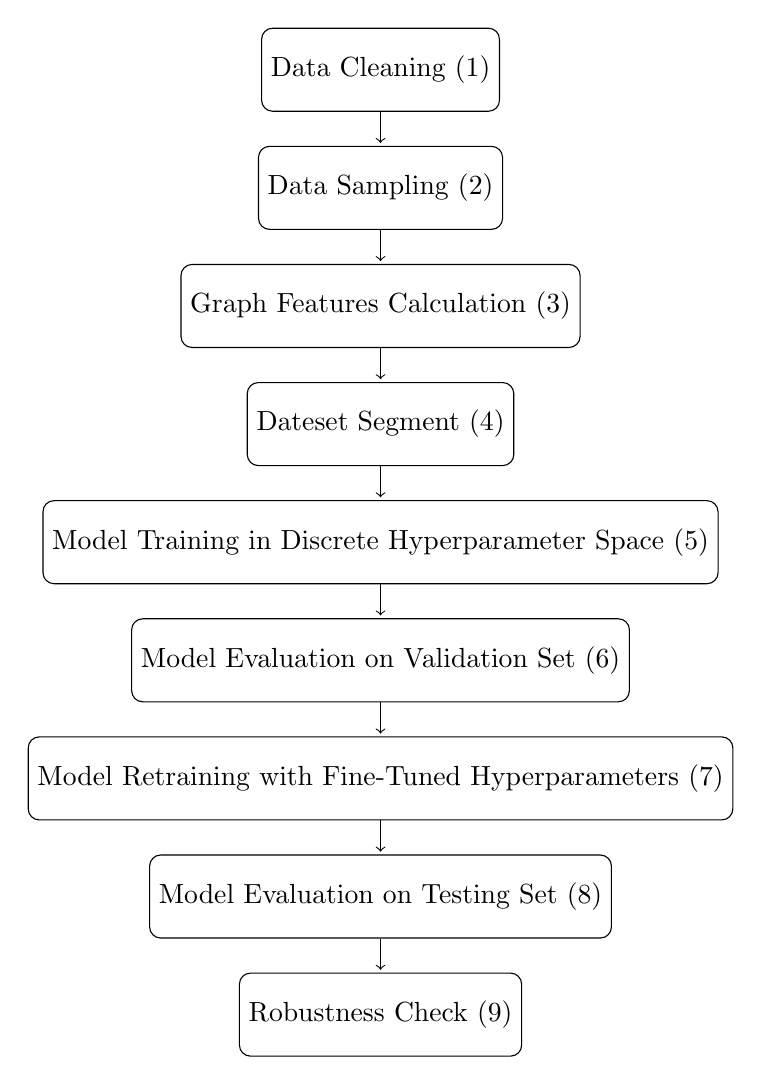
\begin{tikzpicture}[node distance = 1.5cm, auto]
    \node [block] (init) {Data Cleaning (1)};
    \node [block, below of=init] (process1) {Data Sampling (2)};
    \node [block, below of=process1] (process2) {Graph Features Calculation (3)};
    \node [block, below of=process2] (process3) {Dateset Segment (4)};
    \node [block, below of=process3] (process4) {Model Training in Discrete Hyperparameter Space (5)};
    \node [block, below of=process4] (process5) {Model Evaluation on Validation Set (6)};
    \node [block, below of=process5] (process6) {Model Retraining with Fine-Tuned Hyperparameters (7)};
    \node [block, below of=process6] (process7) {Model Evaluation on Testing Set (8)};
    \node [block, below of=process7] (end) {Robustness Check (9)};
    
    \path [line] (init) -- (process1);
    \path [line] (process1) -- (process2);
    \path [line] (process2) -- (process3);
    \path [line] (process3) -- (process4);
    \path [line] (process4) -- (process5);
    \path [line] (process5) -- (process6);
    \path [line] (process6) -- (process7);
    \path [line] (process7) -- (end);
\end{tikzpicture}
\caption{The data modeling workflow.}
\label{fig: data modeling workflow}
\end{figure}

Initial data cleaning serves as the first step of our workflow. At this stage, \revision{we remove columns identified as irrelevant to the default status of a loan, such as \textit{DateOfBirth}. We adjust variables to correct formats, that is, continues value, categorical value, date and string. We delete a list of forward-looking biased variables that cannot be known prior to the target variable and drop these alongside duplicate variables. We} exclude rows containing missing values. Furthermore, columns exhibiting high correlation with other variables, as indicated by the Variance Inflation Factor (VIF), are dropped to reduce multicollinearity. \revision{Most importantly, we create the binary label, \textit{default}, which the model will predict. The definition of \textit{default} is:}
\begin{equation}
y= \textit{default}=
\begin{cases} 
1 & \text{if \textit{DefaultDate} is not null,} \\
0 & \text{otherwise}
\end{cases}
\end{equation}
\revision{which means we regard a loan as defaulted if an interest is not paid on time before the data download date. Otherwise, we regard the loan as non-defaulted.}

Afterwards we perform a sampling procedure to handle the class imbalance in our binary classification task. \revision{In the cleaned dataset, there are 12, 228 default loans and 20, 241 non-default loans. As supervised models usually perform better on a balanced dataset \citep{jing2019multiset}, we randomly sample 12, 000 default loans and 12, 000 non-default loans. Then we construct a network, based on the balanced sample of 24, 000 loans, and calculate graph features by applying methodology introduced in Subsection \ref{subsubsec: Process of Network Construction on Loans}.}

Our dataset is then split into training, validation, and testing sets at a ratio of $0.6:0.2:0.2$. A feature selection procedure is carried out on the training set, removing features where most observations share the same value, as well as graph features that cannot be calculated on the graph in the context of our study. 

Models of three types (EN, RF, MLP) under all respective possible combinations of hyperparameters introduced in Subsection \ref{subsec: ML Models} are subsequently trained on the training set. This is done for two groups of models: the first group is trained only on the initial features, and the second group is trained on both the initial and graph features. 

We then \revision{separately} perform hyperparameter tuning on both model groups using the validation set. The best performing combination of hyperparameters for each model type in each group is afterwards selected based on their performance on the corresponding validation set. \revision{According to the model performance on the validation set, we also delete unimportant features in the dataset. Afterwards we train the models in both groups under the best performing combination of hyperparameters. This is also done on the training set without unimportant features. Then we test models in both groups on the testing set and report the performance.}

Finally, we conduct a robustness check by shuffling the graph features and repeating the steps outlined above. If the performance difference between the two model groups disappears, we conclude that this signifies the observed performance improvement to be indeed attributable to the network centrality features.

\section{Data}
\label{Data}
In this analysis, we employ a holistic dataset acquired from Bondora, a prominent European P2P lending platform based in Estonia, in order to explore the dynamics of loan default. This comprehensive dataset encompasses 32,469 individual borrowers, each of which is detailed through a combination of 155 categorical and continuous variables. This rich set of variables provides a multi-dimensional perspective into the complex factors that could influence loan default risk. \revision{Lending on Bondora is characterized by a diversity of borrowers and lenders, a trait that is inherently captured in our dataset. Borrowers on the platform are largely individuals seeking personal loans, and they encompass a wide array of demographics, credit histories, and borrowing needs.}

\subsection{Dataset Characteristics}

All \revision{credit features} provide valuable context about the borrower's past interactions with the credit market, and by extension, her potential risk profile\footnote{A detailed description of the informative features used for the analysis after the pre-processing of the data sample can be found in \ref{Appendix E}}.


Based on an initial screening process via histograms of each \revision{credit feature} within our dataset, we are able to filter and classify a range of variables that we assume to have a stronger influence on the default classification of an individual \revision{loan}\footnote{The detailed histograms of the most informative loan features of the Bondora dataset can be found in \ref{All_Histo_Infor._loan_feat.}.}. \autoref{Descriptive Statistics for Informative Loan Features (Unbalanced)} provides the summary statistics that disclose the lower moments of these variables in the original dataset. In total, the dataset contains 12,228 defaulted and 20,241 \revision{non-defaulted loans}.

\begin{table}[H]
\centering
\begin{tabularx}{\linewidth}{|l|X|X|X|X|X|}
    \hline
    \footnotesize \textbf{} & \footnotesize \textbf{Count} & \footnotesize \textbf{Mean} & \footnotesize \textbf{Std. Dev.} & \footnotesize \textbf{Min} & \footnotesize \textbf{Max} \\
    \hline
    liab.l & 32469 & 5.11 & 2.08 & 0.00 & 10.48 \\
    inc.total & 32469 & 6.98 & 0.53 & 0.79 & 13.09 \\
    Monthly Payment & 32469 & 4.03 & 0.97 & 0.00 & 7.55 \\
    log. amount & 32469 & 7.28 & 0.92 & 4.66 & 9.27 \\
    time & 32469 & 3.55 & 0.64 & 1.84 & 4.80 \\
    Interest & 32469 & 17.76 & 5.39 & 7.27 & 38.00 \\
    Amt. Prev. Loans Bef. Loan & 32469 & 5317.28 & 6034.19 & 0.00 & 74740.00 \\
    No. Prev. Loans & 32469 & 2.71 & 3.02 & 0.00 & 26.00 \\
    Age & 32469 & 39.63 & 11.46 & 18.00 & 70.00 \\
    \hline 
    \end{tabularx}
\caption{Descriptive statistics for the top 9 informative loan features on the cleaned and unbalanced dataset.}
\label{Descriptive Statistics for Informative Loan Features (Unbalanced)}
\end{table}

\clearpage

From \autoref{Descriptive Statistics for Informative Loan Features (Unbalanced)}, we observe that most of the variables lie within similar ranges.

\revision{Nonetheless, individual borrowers} in our sample, are displaying a wide range of financial backgrounds and borrowing behaviors. For instance, the total income ('inc.total') varies considerably, as shown by its standard deviation of $0.53$ around the mean of $6.98$. Similarly, there's significant variation in the number of previous loans ('No. Prev. Loans'), with some borrowers having as many as $26$ previous loans while others have none.

\revision{Furthermore,} it's noteworthy that borrower \revision{groupings} appear diverse, not limited to any particular age group or credit background. However, the dataset is unbalanced, specifically in the context of our target variable, the individual loan default status. This can pose challenges for statistical learning and prediction accuracy which we will address in \autoref{Methodology} of this article.

Finally, the average interest rate across all loans is $17.76\%$, with a standard deviation of $5.39\%$, indicating a considerable degree of variation in the cost of borrowing. This, along with the other variables, underscores the heterogeneity of our sample and sheds light on the complexity of predicting loan outcomes.

In order to derive at a balanced dataset, containing an equal amount of defaulted versus non-defaulted loans, for the following stages of our methodological approach, we subsequently draw a randomised sub-sample of $24,000$ observations from the original dataset. \autoref{Descriptive Statistics for the Most Informative Loan Features} shows the summary statistics for this particular sub-sample.

\begin{table}[H]
\centering
\begin{tabularx}{\linewidth}{|l|X|X|X|X|X|}
    \hline
    \textbf{} & \textbf{Count} & \textbf{Mean} & \textbf{Std. Dev.} & \textbf{Min} & \textbf{Max} \\
    \hline
    liab.l & 24000 & 5.13 & 2.05 & 0.00 & 10.48 \\
    inc.total & 24000 & 6.96 & 0.52 & 0.79 & 13.09 \\
    Monthly Payment & 24000 & 4.01 & 0.98 & 0.00 & 7.55 \\
    log. amount & 24000 & 7.29 & 0.92 & 4.66 & 9.27 \\
    time & 24000 & 3.53 & 0.63 & 1.84 & 4.80 \\
    Interest & 24000 & 17.72 & 5.37 & 7.29 & 38.00 \\
    Amt. Prev. Loans Bef. Loan & 24000 & 5347.45 & 5914.89 & 0.00 & 74740.00 \\
    No. Prev. Loans & 24000 & 2.75 & 3.03 & 0.00 & 26.00 \\
    Age & 24000 & 39.79 & 11.59 & 18.00 & 70.00 \\
    \hline 
    \end{tabularx}
\caption{Descriptive statistics for the top 9 most informative loan features.\tnote{a}}
\label{Descriptive Statistics for the Most Informative Loan Features}
\end{table}

\subsection{Description of the Six Network-Based Centrality Features}
In addition to the standard variables typically found in P2P lending datasets, our dataset incorporates network-related measures, reflecting our objective to integrate graph theory into credit risk modeling. In \autoref{Descriptive Statistics for the Network Centrality Measures} we present a detailed table of the summary statistics for the computed centrality measures:
\vspace{0.15cm}

\begin{table}[H]
\centering
\begin{tabularx}{0.8\linewidth}{|l|X|X|X|X|X|X|}
    \hline
    \textbf{} & \textbf{Count} & \textbf{Mean} & \textbf{Std. Dev.} & \textbf{Min} & \textbf{Max} \\
    \hline
    PageRank & 24000 & 0.000042 & 0.000026 & 0.000023 & 0.000359 \\
    betweenness & 24000 & 2.589516e-09 & 8.100456e-09 & 0.000000 & 2.153047e-07 \\
    closeness & 15221 & 26.07 & 15.44 & 3.76 & 663.01 \\
    katz & 24000 & 0.01 & 0.00 & 0.01 & 0.01 \\
    authority & 24000 & 0.00 & 0.01 & 0.00 & 0.93 \\
    hub & 24000 & 0.00 & 0.01 & 0.00 & 0.33 \\
    \hline 
    \end{tabularx}
\caption{Descriptive statistics for the network centrality measures.}
\label{Descriptive Statistics for the Network Centrality Measures}
\end{table}

Upon analyzing the computed network centrality features, we find in \autoref{Descriptive Statistics for the Network Centrality Measures} that the mean values for most of these measures are close to zero, thereby indicating that the average loan contract exhibits relatively low centrality within the network. This finding underscores a lower influence and prominence of individual borrowers within the broader loan network, thus showcasing the rather decentralised nature of the P2P loan network in our sample.

\section{Results}
\label{Results}
\subsection{Best Performing Combination of Hyperparameters for Both Groups}
\revision{In this subsection, we elaborate on the hyperparameter combination that results in the optimal performance of our models on the validation set, as delineated in Step 6 of the Figure \ref{fig: data modeling workflow}. The resulting fine-tuned hyperparameter set, displayed in \ref{model_summary}, has been subsequently employed for the retraining of the model, as outlined in Step 7 of the same figure. We report the value for all three types of models in two groups: Group 1 - represents models trained on training set without centrality measures; Group 2 - represents models trained on training set with centrality measures.}
\begin{table}[H]
\centering
    \begin{tabular}{|l|l|l|l|}
\hline
\textbf{Model} & \textbf{Hyperparameter} & \textbf{Group 1} & \textbf{Group 2} \\ \hline
\multirow{4}{*}{EN} & Family & binomial & binomial \\ \cline{2-4} 
& Link  & logit & logit \\ \cline{2-4} 
& $\alpha$ & 0.2 & 0\\ \cline{2-4} 
& $\lambda$ & 0.0001 & 0.0001 \\ \hline

\multirow{5}{*}{RF} & \texttt{ntrees} & 250 & 250 \\ \cline{2-4} 
& Min Depth  & 20 & 20 \\ \cline{2-4} 
& \texttt{max_depth} & 20 & 20 \\ \cline{2-4} 
& Min Leaves & 430 & 659 \\ \cline{2-4} 
& Max Leaves & 2609 & 2463 \\ \cline{2-4} 
& Mean Leaves & 2066.14 & 2090.48 \\ \hline

\multirow{3}{*}{MLP} & \texttt{hidden} & [200, 200] & [200, 100, 200] \\ \cline{2-4} 
& \texttt{epoch}  & 20 & 20 \\ \cline{2-4} 
& \texttt{max_depth} & 10 & 10 \\ \hline

\end{tabular}
\captionsetup{font=scriptsize}
\caption{Best performing combination of hyperparameters.}
\label{model_summary}
\end{table}

\subsection{Model Performance Comparison}
\revision{To thoroughly assess the efficacy of our three models, EN, RF, and MLP, we employ a diverse set of evaluation metrics, as detailed in Subsection \ref{subsec: Model Evaluation}. This comprehensive evaluation is conducted on the testing set, corresponding to Step 8 in Figure \ref{fig: data modeling workflow}, for both model group 1 and group 2.}

\subsubsection{Model Performance Metrics}

\revision{Tables \ref{tab:confusion matrix} and \ref{tab: Model Performance Metrics} encapsulate the comparative performance metrics of the fine-tuned EN, RF, and MLP models on the test dataset. These tables are structured to present a clear differentiation of the model effectiveness with respect to standard metrics including the confusion matrix, accuracy, precision, recall, F1-score, AUC, MSE, and RMSE. We should notice here that the prediction of all models is the probability of default, a continues value between 0 and 1. Thus, the calculation of confusion matrix, accuracy, precision, recall and F1-score is affected by the choice of threshold, while the calculation of AUC, MSE, and RMSE is not. In this subsection, we report the confusion matrix, accuracy, precision, recall and F1-score on testing set when the threshold to maximize the F1-score on training set is applied.}

\begin{table}[H]
\noindent\begin{minipage}{.1\textwidth}
  \centering
  Model
\end{minipage}
\begin{minipage}{.4\textwidth}
  \centering
  Group 1
\end{minipage}
\hspace{1em}
\begin{minipage}{.4\textwidth}
  \centering
  Group 2
\end{minipage}

\vspace{1em}


\noindent\begin{minipage}{0.1\textwidth}
  \centering
  EN
\end{minipage}
\begin{minipage}[t]{.4\textwidth}
  \centering
  \footnotesize
  \setlength\tabcolsep{3pt}
  \begin{tabular}{|l|l|l|l|l|}
    \hline
    & \textbf{0} & \textbf{1} & \textbf{Error} & \textbf{Rate} \\ \hline
    \textbf{0} & 1004 & 1364 & 0.576  &  (1364.0/2368.0) \\ \hline
    \textbf{1} &  311  & 2121 & 0.1279  & (311.0/2432.0) \\ \hline
    \textbf{Total} & 1315 & 3485 & 0.349  &  (1675.0/4800.0)) \\ \hline
  \end{tabular}
\end{minipage}
\hspace{1em}
\begin{minipage}[t]{.4\textwidth}
  \centering
  \footnotesize
  \setlength\tabcolsep{3pt}
  \begin{tabular}{|l|l|l|l|l|}
    \hline
    & \textbf{0} & \textbf{1} & \textbf{Error} & \textbf{Rate} \\ \hline
    \textbf{0} & 1586 & 782&   0.3302 &  (782.0/2368.0) \\ \hline
    \textbf{1} & 423  & 2009 & 0.1739  & (423.0/2432.0) \\ \hline
    \textbf{Total} & 2009  &2791 & 0.251  &  (1205.0/4800.0) \\ \hline
  \end{tabular}
\end{minipage}

\vspace{1em}
\noindent\begin{minipage}{0.1\textwidth}
  \centering
  RF
\end{minipage}
\begin{minipage}[t]{.4\textwidth}
  \centering
  \footnotesize
  \setlength\tabcolsep{3pt}
  \begin{tabular}{|l|l|l|l|l|}
    \hline
    & \textbf{0} & \textbf{1} & \textbf{Error} & \textbf{Rate} \\ \hline
    \textbf{0} & 978  & 1390 & 0.587  &  (1390.0/2368.0) \\ \hline
    \textbf{1} & 212 &  2220&  0.0872 &  (212.0/2432.0) \\ \hline
    \textbf{Total} & 1190 & 3610  &0.3337  & (1602.0/4800.0) \\ \hline
  \end{tabular}
\end{minipage}
\hspace{1em}
\begin{minipage}[t]{.4\textwidth}
  \centering
  \footnotesize
  \setlength\tabcolsep{3pt}
  \begin{tabular}{|l|l|l|l|l|}
    \hline
    & \textbf{0} & \textbf{1} & \textbf{Error} & \textbf{Rate} \\ \hline
    \textbf{0} & 1839&  529  & 0.2234 &  (529.0/2368.0) \\ \hline
    \textbf{1} &  492  & 1940 & 0.2023 &  (492.0/2432.0) \\ \hline
    \textbf{Total} & 2331 & 2469 & 0.2127 &  (1021.0/4800.0) \\ \hline
  \end{tabular}
\end{minipage}

\vspace{1em}
\noindent\begin{minipage}{0.1\textwidth}
  \centering
  MLP
\end{minipage}
\begin{minipage}[t]{.4\textwidth}
  \centering
  \footnotesize
  \setlength\tabcolsep{3pt}
  \begin{tabular}{|l|l|l|l|l|}
    \hline
    & \textbf{0} & \textbf{1} & \textbf{Error} & \textbf{Rate} \\ \hline
    \textbf{0} & 1151 & 1217  &0.5139 &  (1217.0/2368.0) \\ \hline
    \textbf{1} & 332  & 2100&  0.1365 &  (332.0/2432.0)) \\ \hline
    \textbf{Total} & 1483 & 3317 & 0.3227 &  (1549.0/4800.0) \\ \hline
  \end{tabular}
\end{minipage}
\hspace{1em}
\begin{minipage}[t]{.4\textwidth}
  \centering
  \footnotesize
  \setlength\tabcolsep{3pt}
  \begin{tabular}{|l|l|l|l|l|}
    \hline
    & \textbf{0} & \textbf{1} & \textbf{Error} & \textbf{Rate} \\ \hline
    \textbf{0} & 1731 & 637  & 0.269  &  (637.0/2368.0) \\ \hline
    \textbf{1} & 427 &  2005 & 0.1756 &  (427.0/2432.0) \\ \hline
    \textbf{Total} & 2158 & 2642  &0.2217  & (1064.0/4800.0) \\ \hline
  \end{tabular}
\end{minipage}
\caption{Confusion matrix for three types of models in two groups.}
    \label{tab:confusion matrix}
\end{table}

\begin{table}[H]
\centering
    \begin{tabular}{|l|l|l|l|}
\hline
\textbf{Model} & \textbf{Performance Measure} & \textbf{Group 1} & \textbf{Group 2} \\ \hline
\multirow{7}{*}{EN} & Accuracy & 0.65 & 0.75 \\ \cline{2-4} 
& Precision  & 0.61 & 0.72 \\ \cline{2-4} 
& Recall  & 0.87 & 0.83 \\ \cline{2-4} 
& F1-score & 0.72 & 0.77\\ \cline{2-4} 
& AUC & 0.72 &0.84 \\ \cline{2-4} 
& MSE & 0.21 &0.16 \\ \cline{2-4} 
& RMSE  & 0.46 & 0.40 \\ \hline

\multirow{7}{*}{RF} & Accuracy & 0.67 & 0.79 \\ \cline{2-4} 
& Precision  & 0.61 & 0.79 \\ \cline{2-4} 
& Recall  & 0.91 & 0.80 \\ \cline{2-4} 
& F1-score & 0.73 & 0.79\\ \cline{2-4} 
& AUC & 0.76 & 0.88\\ \cline{2-4} 
& MSE & 0.20 &0.15 \\ \cline{2-4} 
& RMSE  & 0.45 & 0.39 \\ \hline

\multirow{7}{*}{MLP} & Accuracy & 0.68 & 0.78 \\ \cline{2-4} 
& Precision  & 0.63 & 0.76 \\ \cline{2-4} 
& Recall  & 0.86 & 0.82 \\ \cline{2-4} 
& F1-score & 0.73 & 0.79\\ \cline{2-4} 
& AUC & 0.75 & 0.86\\ \cline{2-4} 
& MSE & 0.22 & 0.16\\ \cline{2-4} 
& RMSE  & 0.47 & 0.40 \\ \hline

\end{tabular}
\captionsetup{font=scriptsize}
\caption{Model performance metrics.}
\label{tab: Model Performance Metrics}
\end{table}

\revision{In an intra-model comparison, the RF model distinguishes itself with the highest recall values in both groups, suggesting its robustness in identifying positive cases. The EN model, despite not outperforming the other two models, achieves a reliant level of predictive power. This is particularly notable given its simple and linear modeling approach. The MLP model presents a more balanced profile between precision and recall, leading to competitive F1-scores.}

\revision{The inter-group comparison highlights the impact of incorporating centrality measures into the training process. All models in Group 2, which include these measures, demonstrate enhancements in accuracy, precision, and F1-scores compared to their counterparts in Group 1. This suggests that the integration of centrality measures bolsters model prediction capabilities. Notably, the RF model benefits substantially in precision and AUC. Additionally, reductions in MSE and RMSE across all models in Group 2 affirm the positive influence of centrality measures on model performance. On the other hand, while observing a decline in recall for all models in Group 2, it is important to recognize that this is a consequence of the threshold selection strategy aimed at optimizing the overall model performance. Subsequent sections will demonstrate that, despite the lower recall, Group 2 models exhibit superior ROC and AUC results compared to Group 1. The advanced ROC and AUC outcomes provide Group 2 models with the latitude to adjust the threshold, facilitating a tailored balance between false positives and false negatives. This flexibility ensures that the performance enhancements are not merely nominal but translate into pragmatic gains in predictive accuracy.}

\subsection{ROC, AUC and DeLong Test}
Figure \ref{fig:ROC for all models} shows the ROC curve and results of DeLong test for all three types of models in two groups.

\begin{figure}[htbp]
  \centering
  \begin{minipage}{0.32\textwidth}
    \centering
    \includegraphics[clip, trim=0cm 0cm 0cm 1.25cm, width=\textwidth]{GLM (best_result).pdf}
    \caption*{EN}
  \end{minipage}
  \hfill
  \begin{minipage}{0.32\textwidth}
    \centering
    \includegraphics[clip, trim=0cm 0cm 0cm 1.25cm, width=\textwidth]{RF (best_result).pdf}
    \caption*{RF}
  \end{minipage}
  \hfill
  \begin{minipage}{0.32\textwidth}
    \centering
    \includegraphics[clip, trim=0cm 0cm 0cm 1.25cm, width=\textwidth]{DL (best_result).pdf}
    \caption*{MLP}
  \end{minipage}
  
  \caption{ROC curves for all models.}
  \label{fig:ROC for all models}
\end{figure}

\revision{Across all three models within Group 2, we find an elevation in performance that is consistently observed across the entire spectrum of threshold values. Correspondingly, the AUC metrics for these models surpass those of their counterparts in Group 1. The DeLong test corroborates the enhancements, confirming their statistical significance.}


\revision{\subsection{A Comprehensive Comparison of Model Performance}}

\begin{figure}[H]
\hspace{0cm}
    \begin{tikzpicture}
        \tikzstyle{every node}=[inner sep=0pt]
        \node (A) at (-5,5) {\begin{tabular}{|c|c|c|}
                \hline
                Model & Features in Training Set & AUC \\ \hline
                EN & Initial credit features & 0.72 \\ \hline
                RF & Initial credit features & 0.76 \\ \hline
                MLP & Initial credit features & 0.75 \\ \hline
            \end{tabular}};
        \node[above=0.2cm of A] {Models trained on only initial credit features};
        
        \node (B) at (5,5) {\begin{tabular}{|c|c|c|}
                \hline
                Model & Features in Training Set & AUC \\ \hline
                EN & Centrality features & 0.77 \\ \hline
                RF & Centrality features & 0.78 \\ \hline
                MLP & Centrality features & 0.78 \\ \hline
            \end{tabular}};
        \node[above=0.2cm of B] {Models trained on only centrality features};
        
        \node (C) at (0,0) {\hspace{-0.5cm}\includegraphics[width=9cm,clip,trim=0cm 0cm 0cm 1.3cm]{all_model_roc_curves.pdf}};
        \node[below=0.2cm of C] {Hybrid: models trained on initial credit features and centrality features.};
        
        % Draw the horizontal line from A to B
        \draw[line width=0.5mm] (A) -- (B);
        
        % Draw the arrow from the middle of the line AB down to C
        \draw[->, line width=0.5mm] ($(A)!.5!(B)$) -- (C);
    \end{tikzpicture}
    \caption{A comprehensive comparison.}
    \label{fig:A Comprehensive Comparison}
\end{figure}


\vspace{-0.5cm}
\revision{To further corroborate on these findings, figure \ref{fig:A Comprehensive Comparison} presents a detailed comparison of model performances, illustrating the significance of centrality features. The ROC curves in the upper-left corner represent models trained exclusively on initial credit features, whereas the ROC curves in the upper-right corner depict models trained solely on centrality features. It is observed that models relying only on centrality features achieve a similar level of predictive capability as those based solely on initial credit features. Combining both feature groups significantly enhances the performance across all model types. The empirical analysis demonstrates that models trained on a unified dataset comprising of both initial credit and centrality features outperform those confined to individual feature sets. This finding substantiates the assertion that the integration of initial credit and centrality features is instrumental for enhancing predictive performance.}


\revision{Additionally, the final ROC curve plot includes the performance of an XGBoost model with fine-tuned hyperparameters on the testing set, demonstrating that all three model types incorporating centrality measures outperform a contingent ML model. This thorough comparison confirms that the introduced centrality measures contribute positively to predictive accuracy. The improvement of model prediction effect by centrality features is common to all types of models.} 

\vspace{\baselineskip}
\subsection{Feature Importance Analysis}
Our investigation is centered on the evaluation of feature importance, particularly focusing on network centrality measures such as PageRank, betweenness, authoriy- and hub-centrality, katz, and closeness. We employ the methodology discussed in \autoref{Methodology} to elaborate on the significance of the network-based features in credit risk prediction. The following sections will discuss the role of the network centrality features in influencing the performance of our EN, RF, and MLP models, \revision{especially from the feature importance perspective. Figure \ref{fig:ROC for all models} presents the feature importance for all three model types across two groups. Models within Group 1 lack values for centrality features. Nonetheless, for comparative convenience, we continue to enumerate all significant features along the x-axis.}

\begin{figure}[H]
  \centering
  \begin{minipage}{\textwidth}
    \centering
    \includegraphics[clip, trim=0cm 3cm 0cm 6cm, width=\textwidth]{glm_feature_importance.pdf}
    \caption*{EN}
  \end{minipage}
  \hfill
  \begin{minipage}{\textwidth}
    \centering
    \includegraphics[clip, trim=0cm 3cm 0cm 6cm, width=\textwidth]{rf_feature_importance.pdf}
    \caption*{RF}
  \end{minipage}
  \hfill
  \begin{minipage}{\textwidth}
    \centering
    \includegraphics[clip, trim=0cm 3cm 0cm 6cm, width=\textwidth]{dl_feature_importance.pdf}
    \caption*{MLP}
  \end{minipage}
  
  \caption{Feature importance for all models with and without graph-based features.}
  \label{fig:Feature importance for all models}
\end{figure}

The comparison across these three models yields several important observations. While the PageRank feature consistently emerges as an influential predictor in all models, other features such as betweenness show varying levels of importance depending on the specific model type. This variability in feature importance across different models indicates the complex interplay between the data characteristics and model architectures.

It is imperative to reconcile that while these findings shed light on the relative contributions of the various network measures to the model's prediction capability, they do not imply causality \citep{hastie2009}. They merely reflect the relationships within the given dataset and the specific models used \citep{james2013introduction}.

The contrasting ranking of the network-based features across the three ML models underscores the inherent differences in how these algorithms capture and interpret the structure of the data. The EN model, being a linear model, tends to emphasize the direct linear effects of variables on the outcome. It assigns importance based on the degree to which a feature contributes to reducing the prediction error, under the constraints imposed by its regularization term \citep{zou2005regularization}. Hence, features like 'PageRank' and 'closeness' centrality, which may exhibit a more prominent linear relationship with the outcome, are assigned a higher importance.

In contrast, tree-based methods like RF inherently account for higher-order interactions and non-linear relationships between variables \citep{breiman2001random}. This allows them to highlight importance not only based on direct effects but also due to the structural influence a feature might have in relation to other features. Therefore, it is immanent to see a broader set of centrality measures like 'PageRank', 'closeness', and 'katz' receiving high importance.

Similarly to non-parametric tree-based models, neural networks like the MLP model are known for their capability to capture complex non-linear interactions and high-dimensional relationships, attributing importance through the weights learned across multiple layers of the network \citep{hastie2009}.  Consequently, we observe a wider set of network-based features like 'betweenness', 'PageRank', 'katz', and 'closeness' being emphasized.

\subsection{Robustness Checks}
In order to control for potential deficiencies in our model specifications and provide robust model estimates, we added six shuffled dummy centrality features to the data sample and model training process that consisted of randomly rearranged observations of the actually computed network centrality measures. The structure of the dummy features was randomly rearranged to eliminate any dependencies and should consecutively represent white noise in the estimation of the model predictions. Consequently, the inclusion of the shuffled centrality features should not be anymore helpful in predicting loan defaults than a randomly drawn i.i.d sequence \citep{dimpfl2018analyzing}. As introduced in \autoref{Methodology} we additionally trained each model on datasets that only included the conventional credit features in combination with the randomized network centrality features to assess the model performance under the corresponding feature selection. Hitherto, by \textit{apriori} assumption none of the models, trained under the inclusion of the randomized centrality features should detect any meaningful feature importance in the default classification process.

As can be seen in the respective plots (\autoref{fig:ROC for all models with shuffled centrality}) of the ROC and AUC metrics of each ML model type in the corresponding feature configuration with and without randomized network centrality features, the inclusion of the latter to the credit features does not improve the predictive accuracy of any of the used credits scoring models. 

\begin{figure}[htbp]
  \centering
  \begin{minipage}{0.32\textwidth}
    \centering
    \includegraphics[page=2,clip, trim=0cm 0cm 0cm 1.25cm, width=\textwidth]{GLM (best_result).pdf}
    \caption*{EN}
  \end{minipage}
  \hfill
  \begin{minipage}{0.32\textwidth}
    \centering
    \includegraphics[page=2,clip, trim=0cm 0cm 0cm 1.25cm, width=\textwidth]{RF (best_result).pdf}
    \caption*{RF}
  \end{minipage}
  \hfill
  \begin{minipage}{0.32\textwidth}
    \centering
    \includegraphics[page=2,clip, trim=0cm 0cm 0cm 1.25cm, width=\textwidth]{DL (best_result).pdf}
    \caption*{MLP}
  \end{minipage}
  
  \caption{ROC curves for all models with shuffled centrality features.}
  \label{fig:ROC for all models with shuffled centrality}
\end{figure}

Although the respective plot for the linear EN model does not appear to be statistically significant, we can still infer that the randomized network centrality features provide no additional explanatory power for the classification of loan defaults in any of the ML techniques.  

\section{Discussion}
\subsection{Result Analysis and Discussion of the Centrality Measures}
\revision{From our analysis in \autoref{Results} it is possible to observe that the inclusion of the graph-based centrality measures lead to a uniform improvement in prediction accuracy across all tested scoring models. We outline the rationale for such findings in the following: I) Path-based and eigenvector-based measures like betweenness, Katz, and PageRank, measuring global node importance, perform exceptionally well due to their ability in detecting similar loan clusters within the network. PageRank expresses the highest uniform importance across all three model-types and is by definition a measure of node importance that is capable to capture loans that group in clusters of similar risk profiles. Similarly, a high betweenness centrality is signaling that a respective loan acts as a bridge to multiple loan clusters with dissimilar risk profiles, thus yielding information about transitional risk profiles. This information is benefiting, particularly complex non-linear models like the MLP, in being able to better classify defaulted loans from non-defaulted counterparts. Contrarily, Katz centrality allows through its conceptualization to classify the indirect influence of a loan in contrast to the entirety of loans in the similarity network. In addition to capturing cluster information on loans with similar credit profiles, Katz centrality also measures the immediate connection of an individual loan to all other loans in the network with diminishing weights added to loans with more distant connections. This information can signify common risk patterns on broader structural risk within the network for specific credit profiles, from which the scoring models, particularly models with increasing non-linear complexity benefit in the loan default classification process. II) The direct consideration of the network structure and its latent information is inherently captured by closeness centrality which reflects the degree to how related a loan contrast with others within the similarity network. This information conveys details about a loans relative risk positioning, which empowers all tested scoring models in better predicting loan default outcomes. The lower feature importance in the EL model could be traced back to the model's linear character that might not capture more complex dependencies considered in the RF and MLP. 
In a more general sense, it is our premise that the centrality measures help to capture latent loan similarity factors which remain unobserved in a traditional specification model, accounting only for the original input features. Thus, by retrieving such latent information located in the network positioning of the individual loans respectively to other loans originated by the platform, we can further improve the classification accuracy of credit scoring models.}

\subsection{Implications for P2P Lending Platforms and Borrowers}\label{sec:implications}

The findings of this study hold profound implications for P2P lending platforms and their borrowers. \revision{Our comparative study sheds light} on the complex relationships in credit risk data and demonstrate the effectiveness of combining ML models with network-based feature extraction to develop more nuanced credit risk assessment tools.

For P2P lending platforms, enhancing the application of basic ML models like the EN, RF, and MLP with graph-based features can help to facilitate more accurate and robust credit risk assessments. In this study we also introduced a modeling approach that is easy to replicate for P2P lending platforms in that they can simply utilise network analysis prior to the credit scoring process, \revision{and apply the network structure to any current risk frame work implemented without being obliged to systematically retrain underlying scoring models.} The outcome of this study can foster understanding for P2P lending platforms in how the different scoring models perform under the influence of network analysis. Platforms can select or combine ML models that best suit their specific needs and risk tolerance to ultimately provide more accurate and stable credit scores. For borrowers, particularly those with limited credit history or unconventional credit profiles, these advancements in credit risk modeling could mean greater access to credit. As ML models can capture complex patterns and utilize a wider range of data types, borrowers may be evaluated more holistically. This can potentially lower the barrier to credit access, especially for underserved segments, without necessarily compromising the risk management standards of the platform.

\subsection{Limitations and Potential Bias}

While this study provides significant insights into the application of ML and network analysis in credit risk modeling, certain limitations and potential biases still deserve attention.

Our analysis, based on a specific dataset, brings to fore the potential limitations concerning generalizability to other contexts or problem applications. Despite our rigorous data cleaning process and the inclusion of a diverse set of features as well as randomized variants of our network centrality variables, we acknowledge that the specific dataset characteristics could still have affected our results. While we can not completely rule out data-induced influences to have an effect on our modelling approach, we still committed best scholarly practices to rigorously ensure valid results within the scope of our paper.    
Another crucial aspect is the inherent bias-variance trade-off. While tuning the models, we made conscious efforts to balance overfitting and underfitting, yet the risk of over- or under-optimization on the training data at the expense of general performance remains. Nevertheless, we also want to advocate that model optimisation was not the primary goal of this study, hence we acknowledge that the evidence presented may not reflect the true optimal state for each ML model in the given parameter constellation as we rather aimed to demonstrate the significance and importance of considering the intricate network structure for the loan default classification process in P2P lending markets.

\section{Conclusion and Future Research}
\label{Conclusion}

In this study, we conducted a thorough analysis of credit default classification in personal P2P lending markets by utilising an advanced network analysis approach in combination with three state-of-the-art ML models: Elastic Net (EN), Random Forest (RF), and Multi-layer Perceptron (MLP). We \revision{apply} a two-step modeling approach to a comprehensive dataset from the Bondora P2P lending platform composed of various borrower characteristics and credit-related attributes. We further explore the usability of network-derived centrality measures such as PageRank, betweenness, closeness, katz, authority, and hub as prediction-enhancing tools in the credit default classification of P2P loans. By computing the Gower's distance between our initial data points, representing individual \revision{loans}, we first study the intricate network structure of our sample and subsequently derive the network-based centrality features.

Our study findings reveal the crucial role that network centrality measures can fulfill in improving the predictive accuracy of credit scoring models. Across all ML models, we find that centrality features emerge as consistently influential, with PageRank proving to be a key attribute in credit default prediction. In addition, closeness, betweeness and Katz centrality demonstrate consistent importance across all models, simultaneously underlining their relevance as important feature for classifying defaulted loans. \revision{By systematically comparing the different graph-enhanced and conventional model types, we find a uniform improvement in the prediction accuracy of all scoring models. In additionally comparing the graph-enhanced models with a reputable ML technique in form of XGBoost we find further evidence of the model superiority of the graph-based models in accurately predicting credit default. Additional tests with randomly shuffled centrality features confirm the robustness of our findings.}

A notable observation from our study is the need for model-specific feature selection. Some features, including katz, betweennness, and closeness centrality, showed varying levels of importance across different models. This emphasizes the complex relationship between data characteristics and model architectures, suggesting further exploration into optimal feature selection and engineering strategies tailored for each model type. Here we see several promising directions for future research. Firstly, while we have demonstrated the efficacy of elastic net, random forest, and deep learning models in predicting credit defaults, there are several other ML techniques that are yet to be fully explored in this context. For instance, the application of support vector machines, gradient boosting algorithms, and newer deep learning architectures could be investigated. We also encourage future studies to consider the integration of even more diverse data types in credit risk modeling. In addition to financial and non-financial indicators, potential data sources could include alternative data such as text from social media, news sentiment, and other behavioral or psychological indicators. Given the increasing availability of such data, there is substantial scope for researchers to explore how these can be harnessed to improve the accuracy and comprehensiveness of credit risk assessments.

\newpage

\section*{Data Availability}
The data will be made available upon request.

\section*{Acknowledgements}
The authors want to thank Štefan Lyócsa and Tomáš Plíhal from Masaryk University for their invaluable help and comments on the data pre-processing and design of the research methods – specifically related to the model estimations.

We also acknowledge the COST Action CA19130 and COST Action CA21163, under the auspices of the European Cooperation in Science and Technology (COST). COST Actions provide networking opportunities for researchers across Europe, fostering scientific exchange and innovation. This has been particularly beneficial for this research project on financial econometrics. 

Moreover, we would like to express our gratitude to the Swiss National Science Foundation for its financial support across multiple projects. This includes the project on Mathematics and Fintech (IZCNZ0-174853), which focuses on the digital transformation of the Finance industry. We also appreciate the funding for the project on Anomaly and Fraud Detection in Blockchain Networks (IZSEZ0-211195), and for the project on Narrative Digital Finance: a tale of structural breaks, bubbles \& market narratives (IZCOZ0-213370).

Most notably, we are grateful for financial support from the Swiss National Science Foundation under the project Network-based credit risk models in P2P lending markets ($100019E-205487$).

Furthermore, we gratefully acknowledge the support of the Marie Skłodowska-Curie Actions under the European Union's Horizon Europe research and innovation program for the Industrial Doctoral Network on Digital Finance, acronym: DIGITAL, Project No. 101119635.

In addition, our research has benefited from funding from the European Union's Horizon 2020 research and innovation program under the grant agreement No 825215 (Topic: ICT-35-2018, Type of action: CSA). This grant was provided for the FIN-TECH project, a training programme aimed at promoting compliance with financial supervision and technology.

Lastly, we acknowledge the cooperative relationship between the ING Group and the University of Twente. This partnership, centered on advancing Artificial Intelligence in Finance in the Netherlands and beyond, has been of great value to our research.


\newpage

\footnotesize

\bibliographystyle{apa}

\bibliography{reference_paper_1}

\newpage
\appendix
\section{Model Specificity of the Elastic Net}
\label{GLM_model_specificity}

In a logistic regression model, the probability that a binary dependent variable equals a case (e.g., loan default) is modeled as a function of various independent variables (or predictors). Let $Y$ be a binary response variable with $Y_i \in {0,1}$ for $i=1,2,...,n$. Let $\mathbf{X}_i$ denote the vector of predictors for the $i$-th observation. The logistic regression model is given by:

\begin{equation}
\log\left(\frac{P(Y_i=1|\mathbf{X}_i)}{1-P(Y_i=1|\mathbf{X}_i)}\right) = \mathbf{X}_i^T \boldsymbol{\beta}
\end{equation}

where $\boldsymbol{\beta}$ is a vector of coefficients to be estimated.

Elastic net regularization is particularly useful when dealing with correlated predictors. In the context of credit risk modeling, such correlated predictors could be different variables related to a borrower's credit history. The elastic net penalty is controlled by the tuning parameters $\lambda$ and $\alpha$, where $\lambda$ controls the overall strength of the penalty and $\alpha$ controls the balance between L1 and L2 penalties.

In the elastic net logistic regression, the objective is to minimize the following cost function:

\begin{equation}
\min_{\boldsymbol{\beta}} \left\{-\frac{1}{n}\sum_{i=1}^{n}\left[Y_i\mathbf{X}_i^T\boldsymbol{\beta} - \log\left(1+e^{\mathbf{X}_i^T\boldsymbol{\beta}}\right)\right] + \lambda\left[(1-\alpha)||\boldsymbol{\beta}||_2^2/2 + \alpha||\boldsymbol{\beta}||_1\right]\right\}
\end{equation}

where $||\boldsymbol{\beta}||_2^2$ is the L2 norm (Ridge penalty) and $||\boldsymbol{\beta}||_1$ is the L1 norm (Lasso penalty). The tuning parameters $\lambda$ and $\alpha$ are typically chosen via cross-validation.

\section{Model Specificty of the Random Forest}
\label{RF_model_specificity}
The random forest model is an ensemble of decision trees, each of which is constructed using a bootstrap sample of the data. At each node, a random subset of predictors is considered for splitting. The final prediction is an average of the predictions made by each individual tree in the case of regression, or by majority voting in the case of classification.

To describe this in a more formal way, we assume to have a dataset ${(\mathbf{x}i, y_i)}{i=1}^n$ where $\mathbf{x}_i \in \mathbb{R}^p$ represents a vector of predictors and $y_i$ denotes the response variable. 
The random forest generates $B$ trees, and for each $b$-th tree, a bootstrap sample of the data is taken. The tree $f_b$ is then developed according to a recursive procedure that firstly selects $m$ variables at random from the $p$ variables. For each variable, the best binary split is found. The best variable or split among these $m$ variables is then chosen and the node is subsequently divided into two daughter nodes. This recursive process on each daughter node continues until a stopping criterion is met.

The prediction of a random forest is then given by:

\begin{equation}
\hat{f}{rf}(\mathbf{x}) = \frac{1}{B}\sum{b=1}^B f_b(\mathbf{x})
\end{equation}

for regression, and by majority voting among ${f_b(\mathbf{x})}_{b=1}^B$ for classification.

\section{Model Specificity of the Multi-Layer Perceptron}
\label{DL_model_specificity}
The Multi-Layer Perceptron (MLP) is a type of neural network model known for its proficiency in pattern recognition and prediction tasks. An MLP comprises an input layer, one or more hidden layers, and an output layer. Each layer consists of a set of neurons (or nodes), where each neuron in a layer is connected to all neurons in the adjacent layers.

The structure of the MLP used in this study is defined by the number of neurons in the input layer, the number of hidden layers, the number of neurons in each hidden layer, and the number of neurons in the output layer. Given a dataset with $p$ predictor variables, the input layer comprises $p$ neurons. The output layer comprises a single neuron for binary classification problems, as is the case for loan default prediction.

Suppose an MLP has $L$ layers (including input and output layers), with layer $l$ consisting of $n^{[l]}$ neurons. For each neuron $i$ in layer $l$, its output $a_i^{[l]}$ is computed as follows:

\begin{equation}
z_i^{[l]} = \sum_{j=1}^{n^{[l-1]}} W_{ij}^{[l]} a_j^{[l-1]} + b_i^{[l]}, \quad a_i^{[l]} = g^{[l]}(z_i^{[l]}),
\end{equation}

where $W_{ij}^{[l]}$ denotes the weight associated with the connection between neuron $j$ in layer $l-1$ and neuron $i$ in layer $l$, $b_i^{[l]}$ is the bias term for neuron $i$ in layer $l$, and $g^{[l]}(\cdot)$ is the activation function for neurons in layer $l$.

In this study, we employ an MLP model with varied hidden layer configurations and a ReLU activation function in hidden layers. The softmax activation function is used in the output layer for class probability estimation. The MLP model is trained using the backpropagation algorithm, coupled with an optimization algorithm such as stochastic gradient descent.
\clearpage

\section{Histogramms of Centrality Measures based on the Balanced Dataset Before the Pre-Processing Step}
\graphicspath{{Images/}}
\begin{figure}[H]
    \centering
    \includegraphics[width=10cm]{descriptive_stats_pagerank.pdf}
    \captionsetup{font={scriptsize}}
    \caption{Display of the histogramm for the PageRank centrality measure after balancing the dataset. The darker descent represents defaulted loans and lighter descent non-defaulted loans.}
    \label{histo_pr}
\end{figure}

\graphicspath{{Images/}}
\begin{figure}[H]
    \centering
    \includegraphics[width=10cm]{descriptive_stats_betweenness.pdf}
    \captionsetup{font={scriptsize}}
    \caption{Display of the histogramm for the betweeness centrality measure after balancing the dataset.The darker descent represents defaulted loans and lighter descent non-defaulted loans.}
    \label{histo_bet}
\end{figure}

\graphicspath{{Images/}}
\begin{figure}[H]
    \centering
    \includegraphics[width=10cm]{descriptive_stats_closeness.pdf}
    \captionsetup{font={scriptsize}}
    \caption{Display of the histogramm for the closeness centrality measure after balancing the dataset. The darker descent represents defaulted loans and lighter descent non-defaulted loans.}
    \label{histo_clos}
\end{figure}

\graphicspath{{Images/}}
\begin{figure}[H]
    \centering
    \includegraphics[width=10cm]{descriptive_stats_katz.pdf}
    \captionsetup{font={scriptsize}}
    \caption{Display of the histogramm for the katz centrality measure after balancing the dataset. The darker descent represents defaulted loans and lighter descent non-defaulted loans.}
    \label{histo_katz}
\end{figure}

\graphicspath{{Images/}}
\begin{figure}[H]
    \centering
    \includegraphics[width=10cm]{descriptive_stats_authority.pdf}
    \captionsetup{font={scriptsize}}
    \caption{Display of the histogramm for the authority centrality measure after balancing the dataset. The darker descent represents defaulted loans and lighter descent non-defaulted loans.}
    \label{histo_auth}
\end{figure}

\graphicspath{{Images/}}
\begin{figure}[H]
    \centering
    \includegraphics[width=10cm]{descriptive_stats_hub.pdf}
    \captionsetup{font={scriptsize}}
    \caption{Display of the histogramm for the hub centrality measure after balancing the dataset. The darker descent represents defaulted loans and lighter descent non-defaulted loans.}
    \label{histo_hub}
\end{figure}


\clearpage
\section{Histograms of the Most Important Borrower and Loan Features Based on the Original Dataset}
\label{All_Histo_Infor._loan_feat.}

\graphicspath{{Images/}}
\begin{figure}[H]
    \centering
    \includegraphics[width=10cm]{descriptive_stats_raw_data_full (Age).pdf}
    \captionsetup{font={scriptsize}}
    \caption{Display of the histogram for the borrower feature 'Age' in the original dataset. The darker descent represents defaulted loans and lighter descent non-defaulted loans.}
    \label{histo_Age_data_full}
\end{figure}

\graphicspath{{Images/}}
\begin{figure}[H]
    \centering
    \includegraphics[width=10cm]{descriptive_stats_raw_data_full (Amt. Prev. Loans Bef. Loan).pdf}
    \captionsetup{font={scriptsize}}
    \caption{Display of the histogram for the borrower feature 'Amt. Prev. Loans Bef. Loan' in the original dataset. The darker descent represents defaulted loans and lighter descent non-defaulted loans.}
    \label{histo_Amt_Prev_Loans_Bef_Loan_data_full}
\end{figure}

\graphicspath{{Images/}}
\begin{figure}[H]
    \centering
    \includegraphics[width=10cm]{descriptive_stats_raw_data_full (inc.total).pdf}
    \captionsetup{font={scriptsize}}
    \caption{Display of the histogram for the borrower feature 'inc.total' in the original dataset. The darker descent represents defaulted loans and lighter descent non-defaulted loans.}
    \label{histo_inc_total_data_full}
\end{figure}

\graphicspath{{Images/}}
\begin{figure}[H]
    \centering
    \includegraphics[width=10cm]{descriptive_stats_raw_data_full (Interest).pdf}
    \caption{Display of the histogram for the borrower feature 'interest' in the original dataset. The darker descent represents defaulted loans and lighter descent non-defaulted loans.}
    \label{histo_interest_data_full}
\end{figure}

\graphicspath{{Images/}}
\begin{figure}[H]
    \centering
    \includegraphics[width=10cm]{descriptive_stats_raw_data_full (liab.l).pdf}
    \captionsetup{font={scriptsize}}
    \caption{Display of the histogram for the borrower feature 'liab.l' in the original dataset. The darker descent represents defaulted loans and lighter descent non-defaulted loans.}
    \label{histo_liab.l_data_full}
\end{figure}

\graphicspath{{Images/}}
\begin{figure}[H]
    \centering
    \includegraphics[width=10cm]{descriptive_stats_raw_data_full (log.amount).pdf}
    \captionsetup{font={scriptsize}}
    \caption{Display of the histogram for the borrower feature 'log.amount' in the original dataset. The darker descent represents defaulted loans and lighter descent non-defaulted loans.}
    \label{histo_log.amount_data_full}
\end{figure}

\graphicspath{{Images/}}
\begin{figure}[H]
    \centering
    \includegraphics[width=10cm]{descriptive_stats_raw_data_full (MonthlyPayment).pdf}
    \captionsetup{font={scriptsize}}
    \caption{Display of the histogram for the borrower feature 'MonthlyPayment' in the original dataset. The darker descent represents defaulted loans and lighter descent non-defaulted loans.}
    \label{histo_monthly_payment_data_full}
\end{figure}

\graphicspath{{Images/}}
\begin{figure}[H]
    \centering
    \includegraphics[width=10cm]{descriptive_stats_raw_data_full (No. Prev. Loans).pdf}
    \captionsetup{font={scriptsize}}
    \caption{Display of the histogram for the borrower feature 'No. Prev. Loans' in the original dataset. The darker descent represents defaulted loans and lighter descent non-defaulted loans.}
    \label{histo_No_Prev_Loans_data_full}
\end{figure}

\graphicspath{{Images/}}
\begin{figure}[H]
    \centering
    \includegraphics[width=10cm]{descriptive_stats_raw_data_full (time).pdf}
    \captionsetup{font={scriptsize}}
    \caption{Display of the histogram for the borrower feature 'time' in the original dataset. The darker descent represents defaulted loans and lighter descent non-defaulted loans.}
    \label{histo_time_data_full}
\end{figure}
\FloatBarrier

\section{Loan Application Data Features and Descriptions}
\label{Appendix E}
\small
\begin{table}[H]
\begin{tabularx}{\textwidth}{|>{\raggedright\arraybackslash}p{0.20\textwidth}|X|}
\hline
\textbf{Features} & \textbf{Description} \\
\hline
date.start & Date when the loan was issued \\
date.end & Loan maturity date according to the latest loan schedule \\
default & 1 - loan defaulted, 0 - otherwise \\
return & Nominal annual return = $[(\text{Future value of all cash-inflows} + \text{loan amount}) / \text{loan amount}]^{1/(\text{actual loan duration in days}/365)} - 1$ \\
RR1 & Modified Internal Rate of Return - 0 re-investment rate \\
RR2 & Modified Internal Rate of Return - re-investment rate given by return on loans ending 365 days prior to the start of the loan (mean, median, weighted) \\
NPRP & Nominal profit in \% = cash inflows / loan amount - 1 \\
NPRA & Nominal net cash = sum of all cash inflows - loan amount \\
FVCI & Future value of cash inflows - loan amount, re-invested at the return (mean, median, weighted) \\
new & 1 - it is a new customer \\
Age & The age of the loan applicant \\
Gender & 1 - Woman, 0 - Male or couple of undefined \\
Interest & Maximum interest accepted in the loan application \\
MonthlyPayment & Estimated amount the borrower has to pay every month \\
No. Prev. Loans & Number of previous loans \\
Amt. Prev. Loans Bef. Loan & Value of previous loans \\
time & Time index in days = Current date of the loan application - Earliest date of a loan application in the dataset \\
time2 & Square of the time index \\
time3 & Cube of the time index \\
Hour & Application hour (ranging from 0 to 22) \\
weekday & Day of the week (1 for Friday, 2 for Monday, 3 for Saturday, 4 for Sunday, 5 for Thursday, 6 for Tuesday)\\
ver & Method used to verify loan application data (2 for income unverified and cross-referenced by phone, 3 for income verified, 4 for income and expenses verified) \\
lang & Language (1 for Estonian, 2 for English, 3 for Russian, 4 for Finnish, 6 for Spanish) \\
log.amount & Natural log of the loan amount \\
duration & Duration of the loan in months (options include 6, 9, 12, 18, 24, 36, 48, 60 months) \\
use & Loan use - consolidation, real estate, home improvement, business, education, travel, vehicle, other, health, not specified \\
educ & Loan applicant's education - basic education, vocational education, secondary education, higher education, not specified \\
marital & Loan applicant's marital status - married, cohabitant, single, divorced, widow \\
depen & Loan applicant's number of children or other dependents - 0, 1, 2, 3, 4 \\
employ & Loan applicant's employment status - partially employed, fully employed, self-employed, entrepreneur, retiree \\
em.dur & Loan applicant's employment duration - more than 5 years, other, retiree, trial period, less than 1 year, less than 2 years, less than 3 years, less than 4 years, less than 5 years \\
exper & Loan applicant's experience - less than 2 years, less than 5 years, less than 10 years, less than 15 years, less than 25 years, more than 25 years \\
\hline
\end{tabularx}
\caption{Loan application data features and descriptions.}
\end{table}

\begin{table}[H]
\begin{tabularx}{\textwidth}{|l|X|}
\hline
\textbf{Features cont.} & \textbf{Description cont.} \\
\hline
Other & Loan applicant's occupation area \\
Mining & Loan applicant's occupation area \\
Processing & Loan applicant's occupation area \\
Energy & Loan applicant's occupation area \\
Utilities & Loan applicant's occupation area \\
Construction & Loan applicant's occupation area \\
Retail.wholesale & Loan applicant's occupation area \\
Transport.warehousing & Loan applicant's occupation area \\
Hospitality.catering & Loan applicant's occupation area \\
Info.telecom & Loan applicant's occupation area \\
Finance.insurance & Loan applicant's occupation area \\
Real.estate & Loan applicant's occupation area \\
Research & Loan applicant's occupation area \\
Administrative & Loan applicant's occupation area \\
Civil.service.military & Loan applicant's occupation area \\
Education & Loan applicant's occupation area \\
Healthcare.social.help & Loan applicant's occupation area \\
Art.entertainment & Loan applicant's occupation area \\
Agriculture.for.fish & Loan applicant's occupation area \\
homeless & Loan applicant's home ownership type - homeless \\
owner & Loan applicant's home ownership type - owner \\
livingw.parents & Loan applicant's home ownership type - living with parents \\
tenant.pfp & Loan applicant's home ownership type - tenant, pre-furnished property \\
council.house & Loan applicant's home ownership type - council house \\
joint.tenant & Loan applicant's home ownership type - tenant \\
joint.ownership & Loan applicant's home ownership type - joint ownership \\
mortgage & Loan applicant's home ownership type - mortgage \\
encumbrance & Loan applicant's home ownership type - owner with encumbrance \\
inc.princ.empl.no & 1 - has income from a principal employer \\
inc.pension.no & 1 - has income from a pension \\
inc.fam.all.no & 1 - has income from family allowances \\
inc.soc.wel.no & 1 - has income from social welfare \\
inc.leave.no & 1 - has income from leave \\
inc.child.no & 1 - has income from child support \\
inc.other.no & 1 - has income from other sources \\
inc.total & Total income [log(x+1)] \\
no.liab & Loan applicant's number of existing liabilities (0, 1, 2, 3, 4, 5, up to 10) \\
liab.l & Total amount of existing liabilities [log(x+1)] \\
no.refin & Loan applicant's number of liabilities after refinancing (0, 1, 2, 3, 4) \\
inc.support & Loan applicant's income from alimony payments [log(x+1)] \\
FreeCash.d & 1 - has free cash \\
FreeCash.l & Total amount of free cash [log(x+1)] \\
no.previous.loan & Loan applicant's number of previous loans (0, 1, 2, 3, 4, 5, 6, 7) \\
previous.loan.l & Total amount of loan applicant's previous loan amounts [log(x+1)] \\
no.previous.repay & Loan applicant's number of previous early repayments (0, more than 1) \\
previous.repay.l & Total amount of loan applicant's previous loan repayments [log(x+1)] \\
A & Bondora rating - A \\
AA & Bondora rating - AA \\
B & Bondora rating - B \\
C & Bondora rating - C \\
\hline
\end{tabularx}
\caption{Loan application data features and descriptions continued.}
\end{table}
\clearpage


\end{document}